\section{Approximations to the $W_q$ scale function}
Consider a spectrally negative Levy risk process $X = u + ct - S(t)$ and associated Levy measure $\nu$ with $\kappa(s) = s(c- \hat{\bar{\nu}} (s))$ as its Levy-Khintchine representation.\\

Letting $\nu_k = \int_{0}^{\infty} x^k \nu(dx)$ be the moments of the Levy measure. Then one can obtain a power series representation of the Levy exponent in terms of the moments given by
\[
\kappa(s) = s(c- \hat{\bar{\nu}} (s)) = cs + \sum_{k=1}^{\infty} \nu_k \frac{(-s)^k}{k!}.
\]
In the Cramer-Lundberg case where the intensity of the claim arrivals are given by the Poisson parameter $\lambda$, we have $\nu_k = \lambda m_k$ where $m_k$'s are the moments of the claims $C_i$.

One can thus write
\begin{align} \label{WMoments}
\hat{W}_q(s) = \frac{1}{\kappa(s)-q} =  \frac{1}{cs - \sum_{k=1}^{\infty} \nu_k \frac{(-s)^k}{k!} - q}.
\end{align}


\subsection{Pade Approximation}
\label{PadeApproxSection}
We can approximate (\ref{WMoments}) by a Pade approximation of order $[n-1,n]$
\begin{align}
\label{appxW}
\hat{W}_q(s) \approx \frac{P_{n-1}(s)}{Q_{n}(s)} = \frac{\sum_{i=0}^{n-1} a_i s^i}{cs^n + \sum_{i=0}^{n-1} b_i s^i}
\end{align}
for some polynomials $P_{n-1}$, $Q_n$, and some constants $a_i, b_i$, $i=0, \ldots, n-1$.

After the approximation the denominator can be factored as
\[
cs^n + \sum_{i=0}^{n-1} b_i s^i = c(s-\gamma_0) \prod_{i=1}^{n} (s+\gamma_i)
\]
and after a partial fraction decomposition of (\ref{appxW}) we get
\[
\hat{W}_q(s) \approx \frac{C_0}{s-\gamma_0} + \sum_{i=1}^{n} \frac{C_i}{s+\gamma_i}
\]
\[
\Rightarrow W_q(x) \approx C_0 e^{\gamma_0 x} + \sum_{i=1}^{n} C_i e^{-\gamma_i x}
\]

Looking back at the properties of the $W_q$ function in the Cramer-Lundberg case, we can force (\ref{W0}) and (\ref{Wprime0}) by setting $a_{n-1}=1$ and $ b_{n-1} = ca_{n-2} -\lambda - q$
\[
\hat{W}_q(s) \approx \frac{s^{n-1} + \sum_{i=0}^{n-2} a_i s^i}{cs^n + (c a_{n-2} -\lambda - q) s^{n-1} +\sum_{i=0}^{n-2} b_i s^i}.
\]

Since we are fitting two values $W_q(0)$ and $W'_q(0)$ into the Pade approximation, this would be a $[1,2]$ Pade approximant
\[
\hat{W}_q(s) \approx \frac{s + a_0}{cs^2 + (c a_0 -\lambda - q) s +b_0}.
\]

Comparing this with the true value of $\hat{W}_q(s)$,
\[
\hat{W}_q(s) = \frac{1}{\kappa(s)-q} \approx \frac{s + a_0}{cs^2 + (c a_0 -\lambda - q) s +b_0}
\]
\[
\Rightarrow cs^2 +(c a_0 -\lambda - q) s +b_0 \approx (s + a_0)(\kappa(s)-q)
\]
\[
\Rightarrow cs^2 +(c a_0 -\lambda - q) s +b_0 \approx (s + a_0)(cs -\nu_1 s +... -q)
\]
\[
\Rightarrow cs^2 +(c a_0 -\lambda - q) s +b_0 \approx (s + a_0)(cs -\lambda m_1 s  -q)
\]
\[
\Rightarrow a_0 = \frac{1}{m_1} \text{ and } b_0 = -\frac{q}{m_1}.
\]
That is,
\begin{align}
\label{WWprime}
\hat{W}_q(s) \approx \frac{s +  \frac{1}{m_1}}{cs^2 + ( \frac{c}{m_1} -\lambda - q) s -\frac{q}{m_1}}.
\end{align}

We note that the given approximation in (\ref{WWprime}) is the same approximation if we consider the claims to be exponential with $m_1 = \frac{1}{\mu}$, as in (\ref{CLexpo}).\\
\bigskip
The optimal boundary $b*$ for this approximation to the $W_q$ function is thus already been solved.

One can also approximate $W_q$ by a higher order Pade approximant, taking into account only (\ref{W0}).\\
That is, setting $n=2$ and $a_{n-1} = 1$ we have
\[
\hat{W}_q(s) = \frac{1}{\kappa(s)-q} \approx \frac{s + a_0}{cs^2 + b_1 s + b_0}.
\]
\[
\Rightarrow \hat{W}_q(s) \approx \frac{s + a_0}{cs^2 + b_1 s + b_0}.
\]
\[
\Rightarrow cs^2 +b_1 s +b_0 \approx (s + a_0)(\kappa(s)-q)
\]
\[
\Rightarrow cs^2 +b_1 s +b_0 \approx (s + a_0)(cs - \lambda m_1 s + \lambda m_2 \tfrac{s^2}{s} - q)
\]
\[
\Rightarrow a_0 = \frac{2m_1}{m_2}, b_1 = \frac{2c m_1 - 2\lambda m_1^2 - m_2 q}{m_2},
\]
\[
\text{ and } b_0 = -\frac{2m_1 q}{m_2}
\]

Therefore
\[
\hat{W}_q(s) \approx \frac{s +\frac{2m_1}{m_2}}{cs^2 + \lt( \frac{2c m_1 - 2\lambda m_1^2 - m_2 q}{m_2} \rt) s -\frac{2m_1 q}{m_2}}.
\]
This can be rewitten as
\[
\hat{W}_q(s) \approx \frac{s +\frac{1}{\tilde {m}_1}}{cs^2 + \lt( \frac{c}{\tilde{m}_1} - \lambda \frac{m_1}{\tilde{m}_1} -q \rt) s -\frac{q}{\tilde {m}_1}}.
\]
where $\tilde{m}_1 = \frac{m_2}{2m_1}$ is the first moment of the equilibrium density $f_e = \frac{\bar{F}}{m_1}$. This approximation is more commonly known as DeVylder's method (\cite{gerber2008methods}).

\subsection{Laguerre Approximation}
\label{LaguerreSec}
Consider the Laguerre polynomials
\[
L_n(x) = \frac{e^x}{n!} \cdot \frac{d^n}{dx^n}[e^{-x} x^n] = \sum_{k=0}^{n} \binom{n}{k} \frac{(-x)^k}{k!}
\]
for $x \geq 0$, $n=0, 1, \ldots$. These polynomials are orthogonal with respect to the weight $e^{-\frac{x}{2}}$, and for constant $\alpha$, $L_n(\alpha x)$ has Laplace transform given by
\[
\hat{L}_n(s) = \frac{(s-\alpha)^n}{s^{n+1}}, n=0,1, \ldots.
\]

Now, define $W^{(\Phi_q)}_0$ to be the $q=0$ scale function with respect to the Esscher transformed measure $P^{(\Phi_q)}$ (will not be discussed in detail, see (\cite{AA}), (\cite{Kyp})) given by
\[
W_q(x) = e^{x \Phi_q} \cdot W^{(\Phi_q)}_0 (x).
\]
By dividing by $e^{x \Phi_q}$, one removes the unique positive pole of $\hat{W}_q$
\[
\hat{W}_q(s) = \frac{1}{s - \Phi_q} \cdot \widehat{W^{(\Phi_q)}_0} (s)
\]
\[
\Rightarrow (s - \Phi_q)\hat{W}_q(s) = \widehat{W^{(\Phi_q)}_0} (s).
\]
By property of Laplace transforms we also know that
\begin{align*}
W^{(\Phi_q)}_0 (x) &=  e^{-x \Phi_q} \cdot W_q(x)\\
\Rightarrow \widehat{W^{(\Phi_q)}_0} (s) &= \hat{W}_q(s + \Phi_q) = \frac{1}{\kappa(s + \Phi_q) - q}\\
&= \frac{1}{\kappa(s + \Phi_q) - \kappa(\Phi_q)}.
\end{align*}

Following (\cite{abate1998numerical}), one can consider
\begin{align} \label{GW}
G(x) = W^{(\Phi_q)}_0(\infty) - W^{(\Phi_q)}_0 (x)
\end{align}
and approximate using Laguerre polynomials
\begin{align} \label{GB}
G(x) \approx C \sum_{n=0}^{\infty} B_n e^{-\alpha x/2} L_n(\alpha x)
\end{align}
for some chosen constants $C, \alpha$, and coefficients $B_n$ to be solved for. Taking the Laplace transform of (\ref{GW})
\begin{align}
\widehat{G (x)} = \widehat{W^{(\Phi_q)}_0(\infty)} - \widehat{W^{(\Phi_q)}_0 (x)} \nonumber \\
\hat{G}(s)= \frac{W^{(\Phi_q)}_0(\infty)}{s} - \widehat{W^{(\Phi_q)}_0} (s) \nonumber \\
=  \frac{W^{(\Phi_q)}_0(\infty)}{s} - \frac{1}{\kappa(s + \Phi_q) - \kappa(\Phi_q)}. \label{Hcomp1}
\end{align}
Taking the Laplace transform of (\ref{GB}) we have
\[
\hat{G}(s) \approx C \sum_{n=0}^{\infty} B_n \cdot \hat{L}_n(s+\alpha / 2) 
\]
\[
\hat{G}(s) \approx C \sum_{n=0}^{\infty} B_n \frac{(s - \alpha / 2)^n}{ (s+\alpha/2)^{n+1}}.
\]
Some computations yield
\begin{align}
\hat{H}(s) &= (s+\alpha/2) \hat{G}(s) \nonumber \\
& \approx C \sum_{n=0}^{\infty} B_n \frac{(s - \alpha / 2)^n}{ (s+\alpha/2)^{n}} \nonumber \\
\Rightarrow \hat{H} \lt( \frac{\alpha}{2} \cdot \frac{1+z}{1-z} \rt) &= \lt( \frac{\alpha}{1-z} \rt) \hat{G} \lt( \frac{\alpha}{2} \cdot \frac{1+z}{1-z} \rt) \label{Hcomp2} \\
&\approx C \sum_{n=0}^{\infty} B_n z^n \nonumber
\end{align}
upon using the `collocation' transformation $z = \frac{s - \alpha/2}{s + \alpha/2} \iff s = \frac{\alpha}{2} \cdot \frac{1+z}{1-z}$.

Hence we solve for the coefficients $B_n$ by taking the Taylor expansion of $\hat{H} \lt( \frac{\alpha}{2} \frac{1+z}{1-z} \rt)$ which is known to us via (\ref{Hcomp2}) and (\ref{Hcomp1}). The approximation we get for $G$ gives us an approximation for $ W^{(\Phi_q)}_0$. An approximation for $W_q$ is then obtained by multiplying by $e^{x \Phi_q}$.

With regards to the choice of $C$ and $\alpha$, one can do a first order Pade approximation discussed in (\ref{PadeApproxSection}), to obtain an approximation to $W^{(\Phi_q)}_0 (x)$ of the form
\[
W^{(\Phi_q)}_0 (x) \approx W^{(\Phi_q)}_0 (\infty) - C \frac{\alpha}{2} e^{-\frac{\alpha}{2}x}.
\]

\subsection{Example: a Cramer-Lundberg model with exponential mixture jumps of order two}
\label{exCL2}

Consider a Cramer-Lundberg process with $c=1/2$, $\lambda = 29/48$ with claim density given by $f(x) = \frac{8}{29}e^{-x} + \frac{42}{29} e^{-2x}$. To obtain rational values we fix $q=1/16$.

Computing the Levy exponent, one gets
\[
\kappa(s) = \frac{1}{2} s + \frac{8}{48} \lt( \frac{1}{s+1} - 1\rt) + \frac{21}{48} \lt( \frac{2}{s+2} -1 \rt)
\]
which then yields
\[
\hat{W}_q (s) = \frac{1}{\kappa(s) - 1/16} = \frac{24(s+1)(s+2)}{(3s-1)(2s+1)(2s+3)}
\]
\[
= -\frac{6}{11} \cdot \frac{1}{2s+3} - \frac{18}{5} \cdot \frac{1}{2s+1} +\frac{672}{55} \cdot \frac{1}{3s-1}
\]
\[
\Rightarrow W_q(x) = -\frac{3}{11} e^{-3x/2} - \frac{9}{5} e^{-x/2} +\frac{224}{55} e^{x/3}.
\]

\begin{figure}
\caption{Plot of $W_q^{''}$ in \ref{exCL2}}
\begin{center}
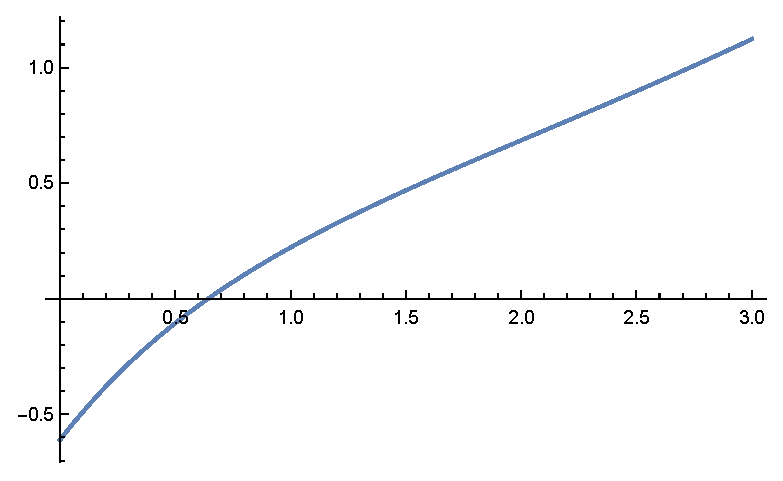
\includegraphics [width=2.8in]{pw2.eps}
\end{center}
\label{pw2}
\end{figure}

A plot of this scale function is given in (\ref{pw2}), and upon doing some calculations one gets the optimal barrier value $b^* = 0.642265$. Furthermore this reveals that the unique positive root $\Phi_q = 1/3$

Doing a Pade [2,3] approximation of $\hat{W}_q$ described in \ref{CLexpo} would yield the exact result (in fact, this is true for all Cramer Lundberg processes with mixed exponential claims of order 2).

Meanwhile, doing the approximation described in (\ref{LaguerreSec}), one first computes
\[
\widehat{W^{(\Phi_q)}_0 (x)} = \frac{8(3s+4)(3s+7)}{s(6s+5)(6s+11)}
\]
which then leads to
\[
\hat{G}(s) = \frac{72(57s+97)}{55(6s+5)(6s+11)}.
\]

\begin{figure}
\caption{Relative errors of the Laguerre approximation in \ref{exCL2}}
\begin{center}
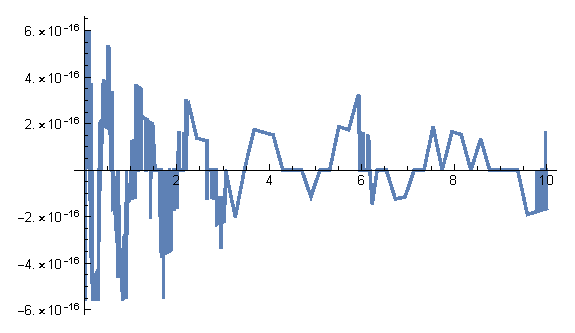
\includegraphics [width=2.8in]{err2.eps}
\end{center}
\label{err2}
\end{figure}

A [0,1] Pade approximation to $\hat{G}$ gives us $\frac{677448}{55(6177s + 5335)}$ implying the Laguerre exponent $\alpha/2 = 5335/6177 = 0.863688$. The resulting error in the Laguerre approximation is plotted in (\ref{err2}), with the largest error being $6*10^{-6}$ when 30 terms are considered in the Laguerre expansion.


